%%
%% This is file `sample-manuscript.tex',
%% generated with the docstrip utility.
%%
%% The original source files were:
%%
%% samples.dtx  (with options: `all,proceedings,bibtex,manuscript')
%% 
%% IMPORTANT NOTICE:
%% 
%% For the copyright see the source file.
%% 
%% Any modified versions of this file must be renamed
%% with new filenames distinct from sample-manuscript.tex.
%% 
%% For distribution of the original source see the terms
%% for copying and modification in the file samples.dtx.
%% 
%% This generated file may be distributed as long as the
%% original source files, as listed above, are part of the
%% same distribution. (The sources need not necessarily be
%% in the same archive or directory.)
%%
%%
%% Commands for TeXCount
%TC:macro \cite [option:text,text]
%TC:macro \citep [option:text,text]
%TC:macro \citet [option:text,text]
%TC:envir table 0 1
%TC:envir table* 0 1
%TC:envir tabular [ignore] word
%TC:envir displaymath 0 word
%TC:envir math 0 word
%TC:envir comment 0 0
%%
%% The first command in your LaTeX source must be the \documentclass
%% command.
%%
%% For submission and review of your manuscript please change the
%% command to \documentclass[manuscript, screen, review]{acmart}.
%%
%% When submitting camera ready or to TAPS, please change the command
%% to \documentclass[sigconf]{acmart} or whichever template is required
%% for your publication.
%%
%%
\documentclass[manuscript,screen,review]{acmart}
%%
%% \BibTeX command to typeset BibTeX logo in the docs
\AtBeginDocument{%
  \providecommand\BibTeX{{%
    Bib\TeX}}}

%% Rights management information.  This information is sent to you
%% when you complete the rights form.  These commands have SAMPLE
%% values in them; it is your responsibility as an author to replace
%% the commands and values with those provided to you when you
%% complete the rights form.
\setcopyright{acmlicensed}
\copyrightyear{2018}
\acmYear{2018}
\acmDOI{XXXXXXX.XXXXXXX}
%% These commands are for a PROCEEDINGS abstract or paper.
%\acmConference[Conference acronym 'XX]{Make sure to enter the correct
%  conference title from your rights confirmation email}{June 03--05,
%  2018}{Woodstock, NY}
%%
%%  Uncomment \acmBooktitle if the title of the proceedings is different
%%  from ``Proceedings of ...''!
%%
\acmBooktitle{Raftian: Pygame Meets Raft,
  TODO 03--05, 2025, Padua, IT}
\acmISBN{978-1-4503-XXXX-X/2018/06}


%%
%% Submission ID.
%% Use this when submitting an article to a sponsored event. You'll
%% receive a unique submission ID from the organizers
%% of the event, and this ID should be used as the parameter to this command.
%%\acmSubmissionID{123-A56-BU3}

%%
%% For managing citations, it is recommended to use bibliography
%% files in BibTeX format.
%%
%% You can then either use BibTeX with the ACM-Reference-Format style,
%% or BibLaTeX with the acmnumeric or acmauthoryear sytles, that include
%% support for advanced citation of software artefact from the
%% biblatex-software package, also separately available on CTAN.
%%
%% Look at the sample-*-biblatex.tex files for templates showcasing
%% the biblatex styles.
%%

%%
%% The majority of ACM publications use numbered citations and
%% references.  The command \citestyle{authoryear} switches to the
%% "author year" style.
%%
%% If you are preparing content for an event
%% sponsored by ACM SIGGRAPH, you must use the "author year" style of
%% citations and references.
%% Uncommenting
%% the next command will enable that style.
%%\citestyle{acmauthoryear}

% Default fixed font does not support bold face
\DeclareFixedFont{\ttb}{T1}{txtt}{bx}{n}{7} % for bold
\DeclareFixedFont{\ttm}{T1}{txtt}{m}{n}{7}  % for normal

% Custom colors
\usepackage{color}
\definecolor{deepblue}{rgb}{0,0,0.5}
\definecolor{deepred}{rgb}{0.6,0,0}
\definecolor{deepgreen}{rgb}{0,0.5,0}
\definecolor{lightpurple}{rgb}{0.6,0.4,0.8}  % New color for comments

\usepackage{listings}

% Python style for highlighting
\newcommand\pythonstyle{\lstset{
language=Python,
basicstyle=\ttm,
morekeywords={self},              % Add keywords here
keywordstyle=\ttb\color{deepblue},
emph={MyClass,__init__},          % Custom highlighting
emphstyle=\ttb\color{deepred},    % Custom highlighting style
stringstyle=\color{deepgreen},
commentstyle=\ttm\color{lightpurple},  % <- This sets comment font and color
frame=tb,                         % Any extra options here
showstringspaces=false,
}}


% Python environment
\lstnewenvironment{python}[1][]
{
\pythonstyle
\lstset{#1}
}
{}

% Python for external files
\newcommand\pythonexternal[2][]{{
\pythonstyle
\lstinputlisting[#1]{#2}}}

% Python for inline
\newcommand\pythoninline[1]{{\pythonstyle\lstinline!#1!}}

\usepackage{fontawesome5}

%%
%% end of the preamble, start of the body of the document source.
\begin{document}

%%
%% The "title" command has an optional parameter,
%% allowing the author to define a "short title" to be used in page headers.
\title{Raftian: Pygame Meets Raft}

%%
%% The "author" command and its associated commands are used to define
%% the authors and their affiliations.
%% Of note is the shared affiliation of the first two authors, and the
%% "authornote" and "authornotemark" commands
%% used to denote shared contribution to the research.
\author{Marco Bellò}
\email{marco.bello.3@studenti.unipd.it}
\author{Tullio Vardanega}
%\authornote{Both authors contributed equally to this research.}
\email{tullio.vardanega@unipd.it}
\orcid{0000-0002-0089-0889}

%\authornotemark[1]

\affiliation{%
  \institution{University of Padua}
  \city{Padua}
  \country{Italy}
}

%%
%% By default, the full list of authors will be used in the page
%% headers. Often, this list is too long, and will overlap
%% other information printed in the page headers. This command allows
%% the author to define a more concise list
%% of authors' names for this purpose.
\renewcommand{\shortauthors}{Bellò and Vardanega}

%%
%% The abstract is a short summary of the work to be presented in the
%% article.
\begin{abstract}
  The problem of shared consensus in a distributed system is both older than a millennium and more relevant than ever: while in the Aegean island of Paxos the challenge was to keep track of the many laws passed in a parliament where legislators had better to do than attend sessions full-time, nowadays the ubiquity of web-based architectures and applications (from a simple cloud storage to the whole banking system) gives daily headaches to developers and system administrators alike.
  To reduce ibuprofen consumption in the IT sector, Ongaro and Ousterhout devised an easily understandable and implementable alternative to the Paxos algorithm, namely the Raft consensus algorithm, which we employ in this work to implement communication via XML-RPC between multiple Pygame applications, each running a game instance that aims to simulate a simplified version of a real-time strategy game. 
\end{abstract}


%%
%% The code below is generated by the tool at http://dl.acm.org/ccs.cfm.
%% Please copy and paste the code instead of the example below.
%%
\begin{CCSXML}
<ccs2012>
   <concept>
       <concept_id>10010520.10010575.10011743</concept_id>
       <concept_desc>Computer systems organization~Fault-tolerant network topologies</concept_desc>
       <concept_significance>500</concept_significance>
       </concept>
   <concept>
       <concept_id>10010147.10011777.10011778</concept_id>
       <concept_desc>Computing methodologies~Concurrent algorithms</concept_desc>
       <concept_significance>500</concept_significance>
       </concept>
   <concept>
       <concept_id>10010147.10010919.10010172.10003824</concept_id>
       <concept_desc>Computing methodologies~Self-organization</concept_desc>
       <concept_significance>500</concept_significance>
       </concept>
   <concept>
       <concept_id>10010147.10010371.10010387.10010391</concept_id>
       <concept_desc>Computing methodologies~Graphics input devices</concept_desc>
       <concept_significance>300</concept_significance>
       </concept>
 </ccs2012>
\end{CCSXML}

\ccsdesc[500]{Computer systems organization~Fault-tolerant network topologies}
\ccsdesc[500]{Computing methodologies~Concurrent algorithms}
\ccsdesc[500]{Computing methodologies~Self-organization}
\ccsdesc[300]{Computing methodologies~Graphics input devices}

%%
%% Keywords. The author(s) should pick words that accurately describe
%% the work being presented. Separate the keywords with commas.
\keywords{Python, Raft, Distribution, Consensus, Gaming, Multiplayer, Multithreading, RPC, Pygame}

\received{TODO}
\received[revised]{TOOD}
\received[accepted]{TODO}

%%
%% This command processes the author and affiliation and title
%% information and builds the first part of the formatted document.
\maketitle

\section{Introduction}

From sharing spreadsheets between a handful of laptops in a small basement office, through large-scale rendering on a supercomputer, to the entire global finance system, distributed computing has become an essential component of the modern world that we almost take for granted: nowadays, what most people need a computer for can be done in the browser thanks to services like email clients, cloud calendars, media streaming platforms and web-based office suites (like Google Docs) that expose word editors, spreadsheets managers, presentations programs and more, all while being constantly synchronized to the cloud, which not only ensures data persistence and availability, but also enables sharing and collaboration between users. 

It does not end here: other examples of distributed applications include cloud storage services like Dropbox, Google Drive or OneDrive, streaming services like Netflix, YouTube or Spotify, distributed computing like blockchain technologies or AWS, online banking services (the banking system itself is distributed since way before), social networks, and even maritime and aircraft traffic control systems.
Moreover, the rise of the gaming industry played a significant role in pushing forward distribution: in 2024 the gaming market revenue was estimated to be $187.7$ billion U.S. dollars \cite{newzoo}, making it a hefty slice of the pie that is the entertainment industry \cite{pwc}, with $111$ billions generated by free-to-play games \cite{f2prevenue} ($70$ billions from social and casual games alone\cite{casualgames}), which interests us since their business model often relies on cosmetics, game passes and advertisements, forcing them to be constantly on-line. 


Let's now define what distribution \textit{is}: a distributed system is a computer system whose inter-communicating components are located on different networked computers \cite{tanenbaum2017distributed} \cite{Apt2009}, which coordinate their actions via message-passing to achieve a common goal. There are three significant challenges to overcome: maintaining components' concurrency \footnote{Concurrency refers to the ability of a system to execute multiple tasks through simultaneous execution or time-sharing (context switching), sharing resources and managing interactions. It improves responsiveness, throughput, and scalability \cite{OSconcepts} \cite{computerOrganization} \cite{george_coulouris_distributed_2012} \cite{parallelComputing} \cite{parallelDistributedHandbook}.}, eliminating global-lock reliance and managing the independent failure of components, all while ensuring scalability (often the purpose is scaling itself) and transparency to the user, meaning interactions with any exposed interface must be done while being unaware of the complexity behind them.

Most importantly, shared consensus must be guaranteed: it does not require much thought to see that all servers in a cluster should agree on one or more shared values, lest becoming a collection of un-related components that have little to do with collaboration (thus distribution). In the most traditional single-value consensus protocols, such as Paxos \cite{paxos}, cooperating nodes agree on a single value (e.g., an integer), while multi-value alternatives like Raft \cite{raft} aim to agree on a series of values (i.e., a log) growing over time forming a sort-of cluster's history. It is worth noting that both goals are hindered by the intrinsically asynchronous nature of real-world communication, which make it impossible to achieve consensus via deterministc algorithms, as stated by Fischer, Lynch and Paterson in their FLP impossibility theorem \cite{flp}. Thankfully this can be circumvented by injecting some degree of randomness.

The concepts and examples we mentioned so far allow us to finally present the goal of this project: we will create a simplified clone of Travian \footnote{Travian: Legends is a persistent, browser-based, massively multiplayer, online real-time strategy game developed by the German software company Travian Games. It was originally written and released in June 2004 as "Travian" by Gerhard Müller. Set in classical antiquity, Travian: Legends is a predominantly militaristic real-time strategy game. Source: \url{https://www.travian.com/international}}, an old real-time \footnote{Real-time games progresses in a continuous time frame, allowing all players (human or computer-controlled) to play at the same time. By contrast, in turn-based games players wait for their turn to play.} player-versus-player \footnote{Player-versus-player (PvP) is a type of game where real human players compete against each other, opposed to player-versus-environment (PvE) games, where players face computer-controlled opponents.} strategy game \footnote{Strategy video game is a major video game genre that focuses on analyzing and strategizing over direct quick reaction in order to secure success. Although many types of video games can contain strategic elements, the strategy genre is most commonly defined by a primary focus on high-level strategy, logistics and resource management. \cite{rollings2003andrew}}, where players build their own city and wage war on one another (less wrinkly readers may be more familiar with the modern counterpart Clash of Clans \footnote{Clash of Clans: \url{https://supercell.com/en/games/clashofclans/}}), built with Pygame \footnote{Pygame: \url{https://www.pygame.org/docs/}}, a Python library that creates and manages all necessary components to run a game such as game-engine, graphical user interface, sounds, plyer inputs and the like, where each player resides in a separate server (or node) that communicate with the others via an algorithm modelled after Raft's specifications. 

This choice follows the author's interest in exploring Raft capabilities and ease of implementation in a fun and novel way, using a language that while extremely popular is seldom used in such a fashion.\\
Both game and algorithm implementations have been reduced to a reasonably complex proof of concept to keep the project scope manageable: it is possible to instantiate games up to five players, each of which is restricted to the only action of attacking the others, while Raft's functionalities are limited to log replication and overwriting. \\
Experiments were conducted to evaluate both game responsiveness and the communication algorithm correctness. \\
All source code is visible at the following link: \url{https://github.com/mhetacc/RuntimesConcurrencyDistribution/blob/main/raftian/raftian.py}.

\section{Python} \label{sec:python}

We will now discuss the technologies employed in the development of the project (section \ref{sec:python}) as well as presenting our implementation of the algorithm Raft.

Python is a high-level, dynamically typed and interpreted programming language that is often used for scripting, data analysis and developing small applications, making it a non-obvious choice for this project, which does not fall into any of these categories.

As a language, it has two main advantages compared to others: first of all it is undoubtedly the most popular and widely used in the world (figure \ref{fig:tiobe}) \cite{tiobe,ieeeSpect} which translates to abundant documentation and resources, and secondly it has a huge ecosystem of libraries that implement all the functionalities we need for this project, namely: \textit{xmlrpc} for the remote procedure calls (RPCs), \textit{threading} to handle local concurrency and \textit{Pygame} to manage everything game-related.

\begin{figure}[h]
  \centering
  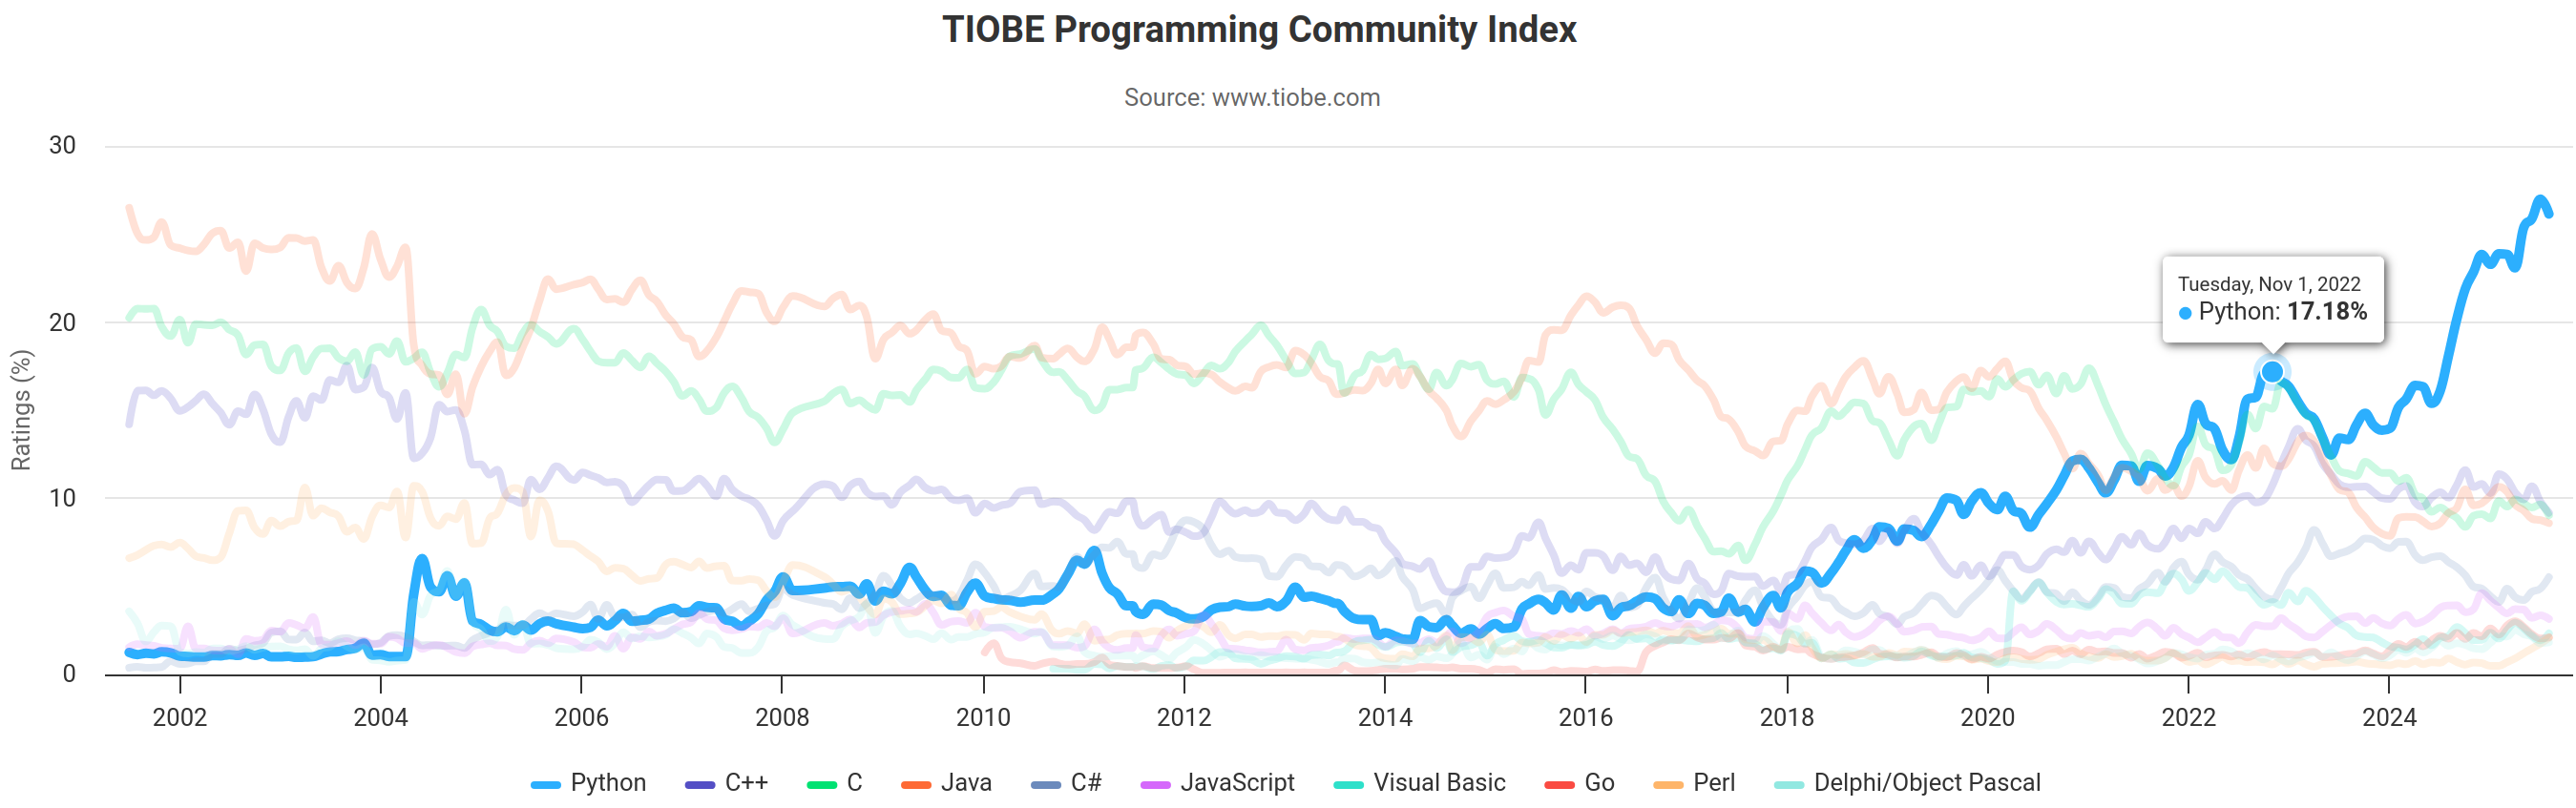
\includegraphics[width=\linewidth]{images/TIOBEindex.png}
  \caption{TIOBE Programming Community Index, focus on Python statistics, 2025. (\url{https://www.tiobe.com/tiobe-index/})}
  \Description{Graph shows that Python gained populary since 2018 onwards becoming the most popular programming language.}
  \label{fig:tiobe}
\end{figure}


\subsection{Remote Procedure Calls} \label{sec:xmlrpc}

In Raft's specifications it is stated that nodes communicate with each other via remote procedure calls \cite{raft}, which in distributed computing is when a program causes a procedure (or subroutine) to execute in another address space (commonly on another computer on a shared network) calling it as if it were local (that is, the programmer writes the same code whether the subroutine is local or remote).

There are many libraries that implement this functionality, like gRPC (\url{https://grpc.io/}) which is a high performance open source RPC framework used by many big players, such as Netflix \footnote{Netflix Ribbon is an Inter Process Communication library built in software load balancers: \url{https://github.com/Netflix/ribbon}} and Cockroach Labs \footnote{Cockroach Labs is the company behind CockroachDB, a highly resilient distributed database: \url{https://www.cockroachlabs.com/}}, available for many languages (Python included), but we opted for the standard library \textit{xmlrpc} \footnote{XML-RPC is a Remote Procedure Call method that uses XML passed via HTTP as a transport: \url{https://docs.python.org/3/library/xmlrpc.html}} thanks to its promised simplicity and ease of use. 

The library provides both server and client implementations, encapsulating the former in its own loop, while the latter can be fired as needed allowing a bit more flexibility in its usage.

In code \ref{code:client}, \verb|client| is an instance of \verb|ServerProxy|, which acts as the client-side interface for XML-RPC, allowing you to call the remote procedure \verb|test_foo| as if it were a local function, even though it executes on a server in a different networked location.

\begin{python}[label={code:client}, caption={Client as server proxy}]
with xmlrpc.client.ServerProxy('http://localhost:8000', allow_none=True) as client:
    print(client.test_foo(42)) # print returned value
\end{python}

The server must be instantiated and kept running by calling its event loop (e.g., using \verb|serve_forever|), and all remote procedure calls must be registered using the \verb|register_function| method of \verb|SimpleXMLRPCServer| (code \ref{code:server}).

\begin{python}[label={code:server}, caption={Server}]
with SimpleXMLRPCServer (('localhost', 8000)) as server:
    def test_foo(number):
        return f'The number is {number}'

    server.register_function(test_foo)  
    server.serve_forever() # keep server alive
\end{python}

For this project, we extended \textit{SimpleXMLRPCServer} to create a class that implements the Raft protocol (more details in section \ref{sec:raft})

\subsection{Concurrency} \label{sec:threading}

In this project the need for concurrent programming arises from two challenges: every server have an internal timer that fires at certain intervals, and every node has to run a game engine and the server itself at the same time, both of which can be simplified as two \textit{"while true"} loops. 

Most Raft implementations achieve concurrency with asynchronous programming, using libraries such as \textit{asyncio} \footnote{asyncio is a library to write concurrent code using the async/await syntax: \url{https://docs.python.org/3/library/asyncio.html}}, which while powerful and efficient, makes writing code a bit awkward and cumbersome. We thus opted for a more traditional approach using multithreaded programming: in computer science, a thread of execution is the smallest sequence of programmed instruction that can be managed independently by the scheduler \cite{lamportMultiprocessor}, and multiple threads may be executed concurrently sharing resources such as memory, which is directly counterpointed to multiprocessing where each process has its own storage space (moreover, processes are typically made of threads). 

In Python there are modules in the standard library for both of them, respectively \textit{threading} \footnote{The threading module provides a way to run multiple threads (smaller units of a process) concurrently within a single process: \url{https://docs.python.org/3/library/threading.html}} and \textit{multiprocessing} \footnote{The multiprocessing module is a package that supports spawning processes using an API similar to the threading module: \url{https://docs.python.org/3/library/multiprocessing.html}}. It is fundamental to note that the former does not provide real multi-threading since, due to the Global Interpreter Lock of CPython (the, for want of a better word, "official" Python implementation), only one thread can execute bytecode at once. To cite directly from the documentation: \textit{"[GIL is] The mechanism used by the CPython interpreter to assure that only one thread executes Python bytecode at a time. This simplifies the CPython implementation by making the object model (including critical built-in types such as dict) implicitly safe against concurrent access. Locking the entire interpreter makes it easier for the interpreter to be multi-threaded, at the expense of much of the parallelism afforded by multi-processor machines."} \footnote{Global Interpreter Lock: \url{https://docs.python.org/3/glossary.html\#term-global-interpreter-lock}}.

Thankfully, this does not apply with the \textit{multiprocessing} module, which creates separate processes instead, offering both local and remote concurrency effectively side-stepping the Global Interpreter Lock, allowing programmers to fully leverage multiple cores. As previously stated, processes are much heavier than threads and thus more expensive to create, but do not incur the risks of shared memory. 

\subsubsection{Comparison}

To evaluate which of the two modules is more suited for our purposes, we devised a simple experiment: we created two game instances with one hundred and one thousands coloured dots respectively (figure \ref{fig:randomdots}), that move around the screen offsetting their position each frame by a random amount between minus five and plus five pixels (pseudocode \ref{code:randomdots}).

Then we ran both of them in various scenarios: with the game instance alone (baselines), with a server alive in a thread and with a server alive in a process, and we measured the \textit{frames per second} (FPS) \footnote{Frame rate, most commonly expressed in frames per second or FPS, is typically the frequency (rate) at which consecutive images (frames) are captured or displayed. This definition applies to film and video cameras, computer animation, and motion capture systems, while in the context of computer graphics is the rate at which a system, particularly the graphic card, si able to generate frames. Source: \url{https://en.wikipedia.org/wiki/Frame_rate}} in each case, since it is the most common metric to evaluate game performance. Higher FPS-count translates to a smoother and more responsive, i.e., better, gaming experience.

\begin{python}[label={code:randomdots}, caption={Pygame graphical dot}]
# create random offsets for both x and y coordinates
xmov = random.randint(-5,5)
ymov = random.randint(-5,5)

# move the dot by a certain offset
dot.move_by(xmov, ymov)
\end{python}

\begin{figure}[h]
  \centering
  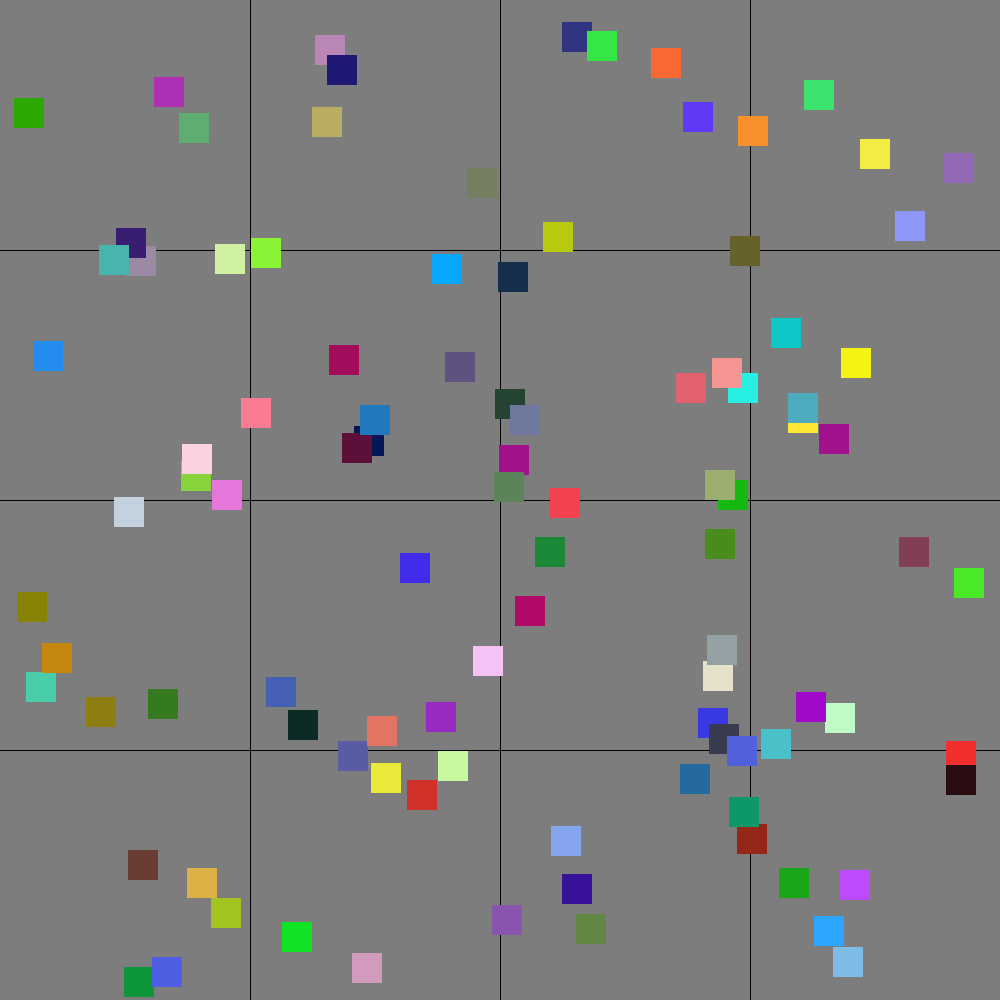
\includegraphics[width=.4\linewidth]{images/100dots.png}
  \hspace{.05\linewidth}
  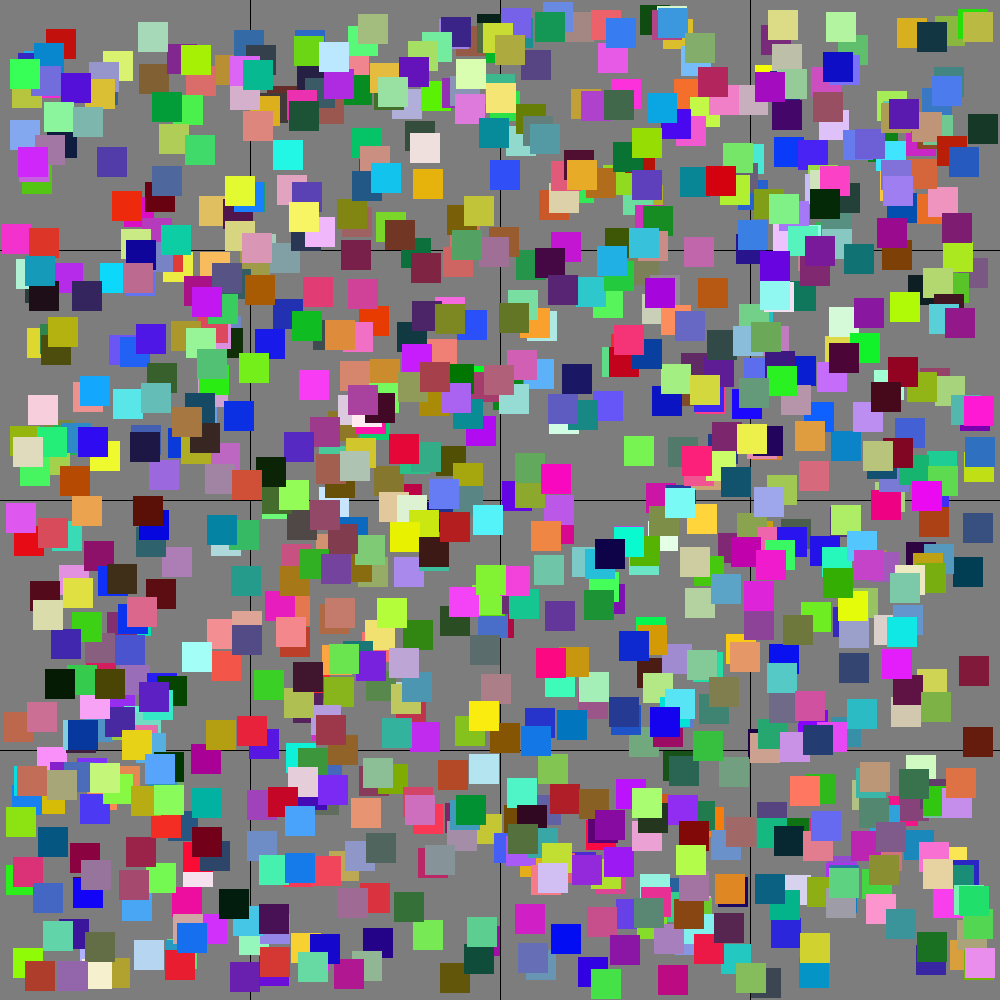
\includegraphics[width=.4\linewidth]{images/1000dots.png}
  
  \caption{Two game instances made with Pygame, with respectively 100 and 1000 dots that randomly move around}
  \Description{Graph shows two game instances with respectively 100 and 1000 little colored squares that, once fired up, move around by a random offset.}
  \label{fig:randomdots}
\end{figure}

Results, shown in the graph at figure \ref{fig:peval} shows us that: 

\begin{itemize}
    \item Increasing the number of dots from 100 to 1000 halves the FPS count;
    \item Adding a server in a separate thread halves performances;
    \item Using \textit{multiprocessing} yields worse performances than \textit{threading} in the 100-dots scenario (about -30\%) while performs similarly in the 1000-dots one.
\end{itemize}

This leads us to conclude that, for our specific purposes, the \textit{threading} module is the best choice, especially since the final game will be way less computationally expensive from a graphical standpoint, hence using a lighter weight alternative should be even more beneficial than tested.

\begin{figure}[h]
  \centering
  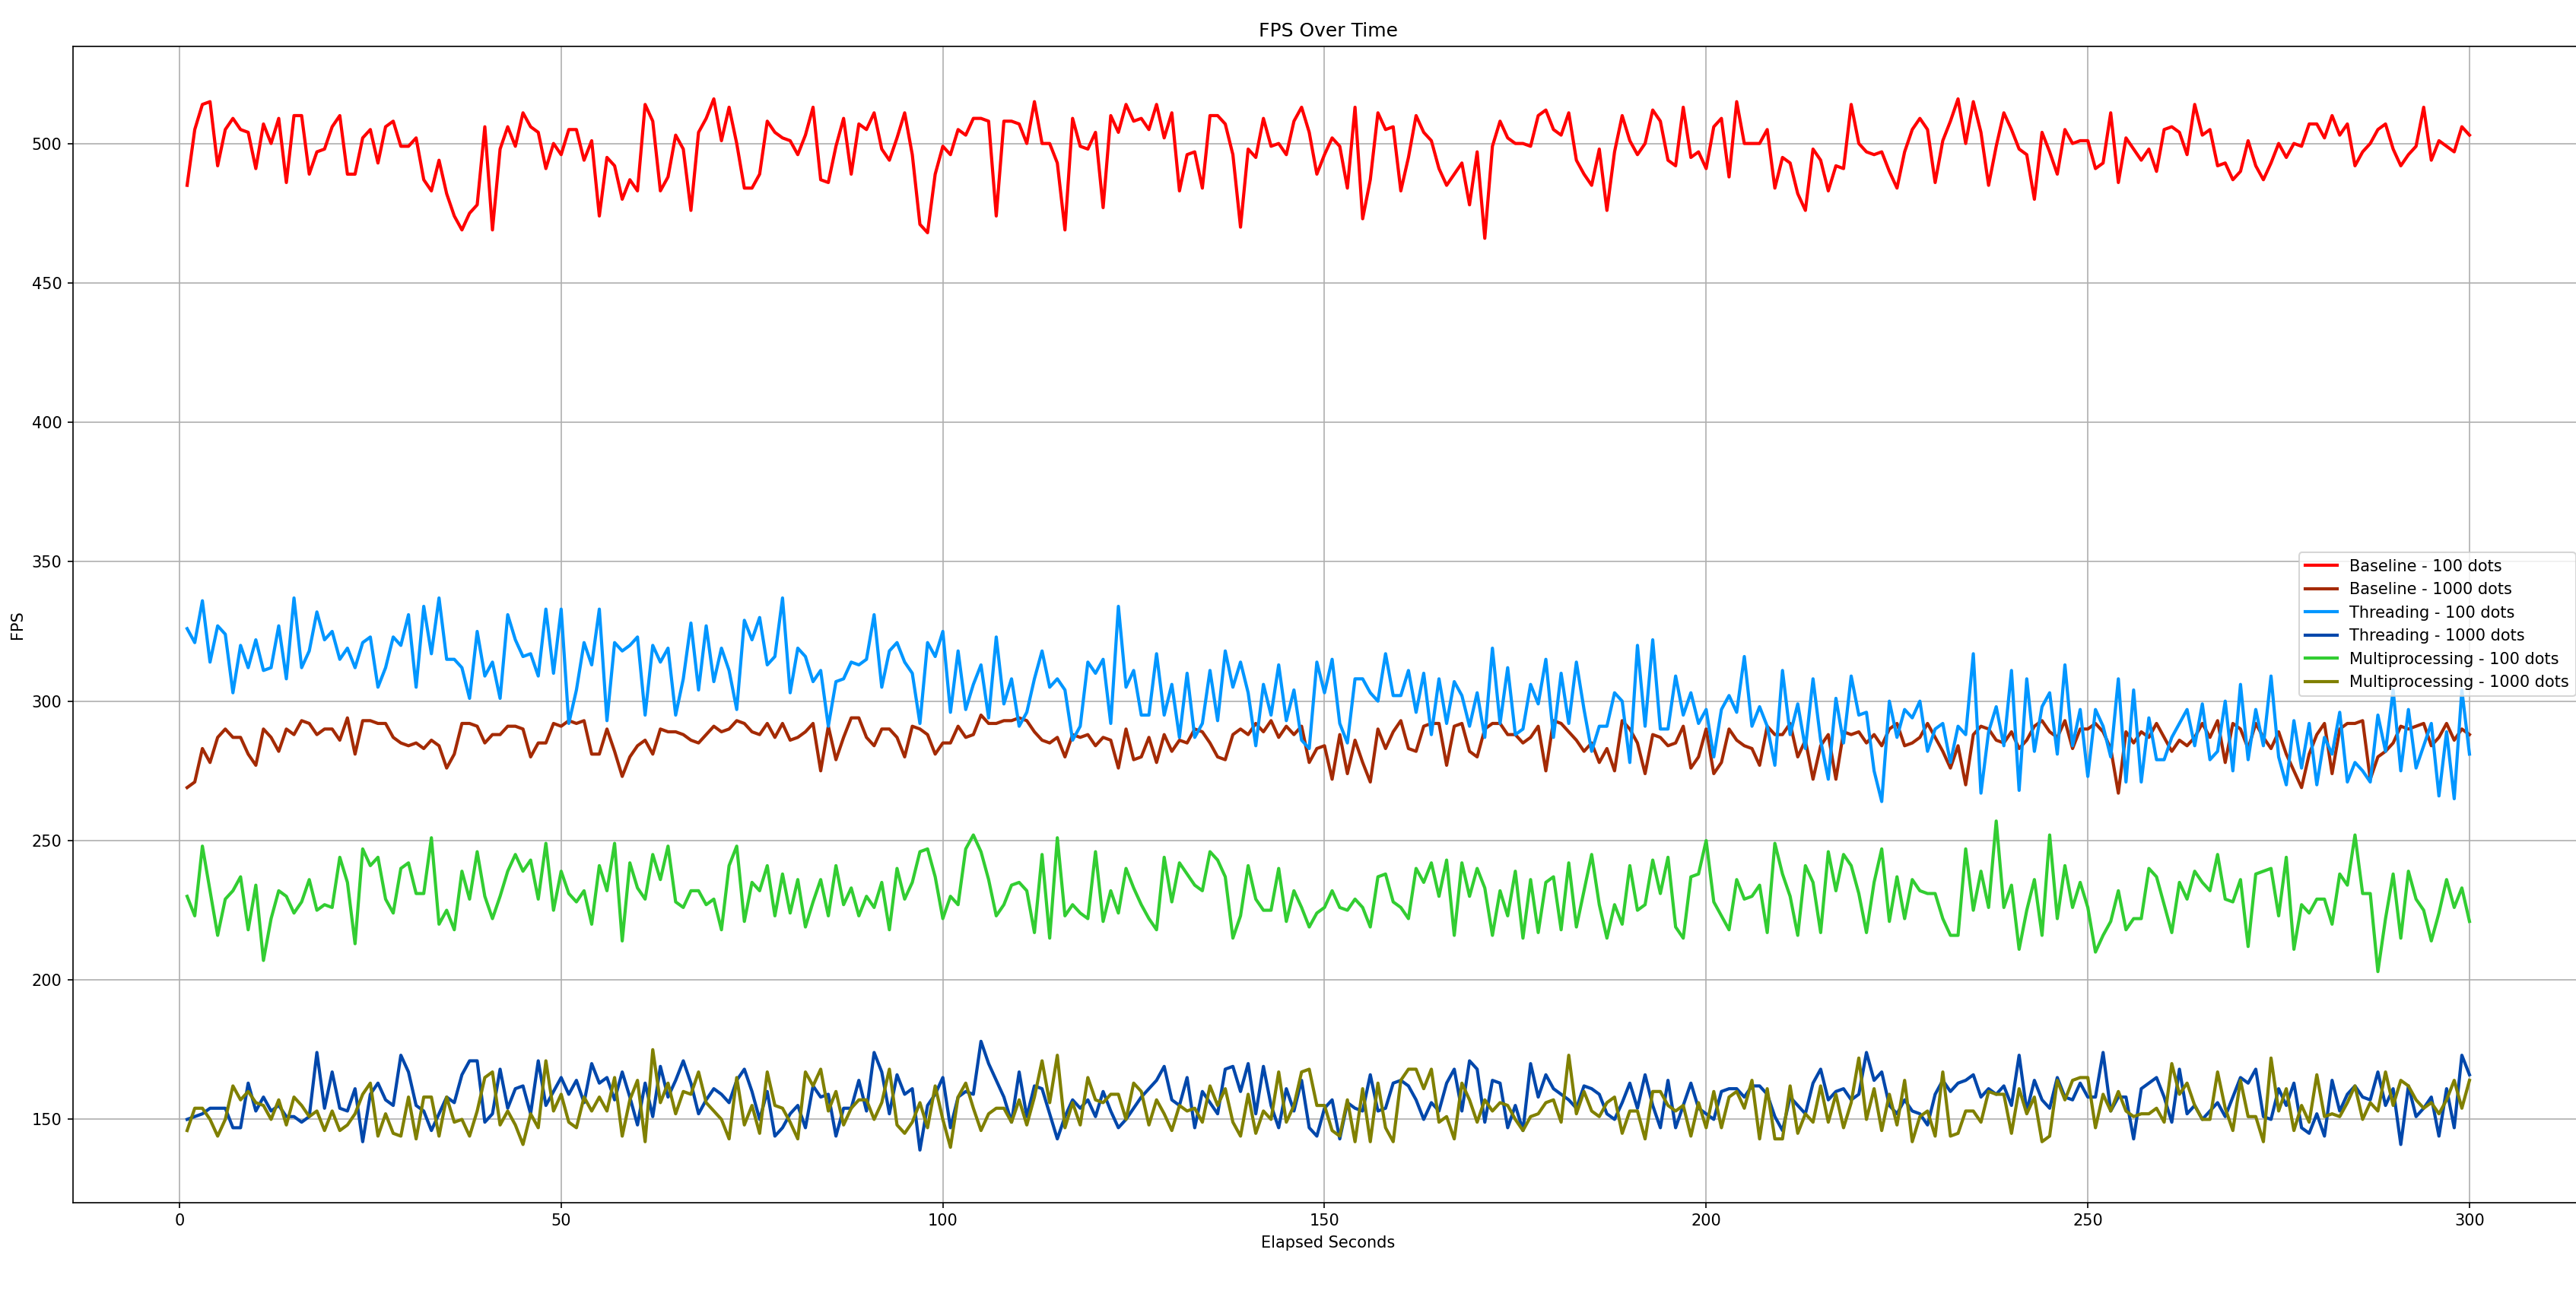
\includegraphics[width=\linewidth]{images/performance_eval_fps_graph.png}
  \caption{Performance evaluation graph: red hues for baselines, blue hues for threading and green hues for multiprocessing. Darker shades for 1000 dots and lighter shades for 100 dots game instances}
  \Description{Line graph that shows that increasing the graphical load by 10x halves performances, and that module trheading performs 30\% better than multithreading in a low-demanding scenario.}
  \label{fig:peval}
\end{figure}

All tests have been performed with the following machine: 

\begin{itemize}
    \item OS: Ubuntu 24.04.1 LTS x86\_64;
    \item Kernel: 6.8.0-52-generic;
    \item Shell: bash 5.2.21;
    \item CPU: 13th Gen Intel i7-13620H;
    \item GPU: NVIDIA GeForce RTX 4050 Laptop GPU;
    \item Memory: 15610MiB;
    \item Python version: 3.12.3;
    \item Power Mode: Balanced;
    \item Power Supply: 100W via type C.
\end{itemize}

\subsection{Game Engines} \label{sec:pygame}

There are many ways to implement a graphical user interface: from clever shell tricks like htop \footnote{htop is a cross-platform text-mode interactive process viewer: \url{https://htop.dev/}}, to full fledged game engines like Unity \footnote{Unity is a cross-platform game engine developed by Unity Technologies: \url{https://unity.com/}} or Godot \footnote{Godot is a cross-platform open-source game engine: \url{https://godotengine.org/}} that often come with their own editor and a \textit{top-down} approach, meaning build the UI first and then go down to code as needed for scripting and refining.

Unfortunately our needs are quite opposite: what we want is a code-only, mono-language framework that while slowing down game development should simplify merging Raft with it. The choice thus boiled down to two alternatives: tkinter and Pygame. 

\subsubsection{Comparison}

Let's list strengths and weaknesses of the two.

\begin{itemize}
  \item \textbf{tkinter:} 
    \begin{itemize} 
      \item \faThumbsUp[regular] Module of the standard library;
      \item \faThumbsUp[regular] Few lines of code to make simple UIs;
      \item \faThumbsDown\ Low flexibility;
      \item \faThumbsDown\ No game loop;
      \item \faThumbsDown\ Not a game engine;
    \end{itemize}
  \item \textbf{Pygame:}
    \begin{itemize}
      \item \faThumbsUp[regular] Extreme flexibility;
      \item \faThumbsUp[regular] Direct access to game loop;
      \item \faThumbsUp[regular] APIs to access many kinds of user inputs;
      \item \faThumbsDown\ Verbose to obtain simple UIs;
      \item \faThumbsDown\ Non-standard community-made framework.
    \end{itemize}
\end{itemize}

We ultimately decided to opt for Pygame for four reasons: it is extremely flexible, exposes many useful functions (for example to catch different user inputs), gives direct access to the game loop and it is a novel and fun framework that has never, to the best of our knowledge, been used in such a fashion. 

\section{Raft} \label{sec:raft}

It is not our intention to plagiarize Ongaro and Ousterhout's excellent work "In Search of an Understandable Consensus Algorithm" \cite{raft} by presenting the Raft algorithm's specifications. Instead, we will discuss how we interpreted and implemented it to mold it into our own use case

The algorithm uses three types of nodes, namely \textit{leader}, \textit{follower} and \textit{candidate}, and revolves around three core functionalities: leader election, log replication and cluster membership change. Log compaction is also mentioned, while a byzantine fault tolerant variant is never explored by the original authors.

One last component, instrumental to the functioning of the algorithm, is the \textit{term}: everything happens in a certain term, which divides time logically and increments every election. 

Our Raft class directly extends \textit{simpleXMLRPCServer} from XML-RPC module, as shown at code \ref{code:raft}.

Lastly, to fire off non-blocking concurrent RPCs on the cluster, we leverage the \textit{concurrent.futures} module using \textit{ThreadPoolExecutor}. To avoid having to keep creating and destroying pools every time a server needs to communicate with the cluster, we embedded a finite amount of workers as class attributes (code \ref{code:threadPool}).

\begin{python}[label={code:raft}, caption={Class Raft definition}]
class Raft(SimpleXMLRPCServer):
    def __init__(self, 
                 addr: tuple[str, int],
                 allow_none: bool = True,
                 # ...
                 last_index_on_server: list[tuple[int, int]] | None = None
                 ):
        SimpleXMLRPCServer.__init__(self, addr=addr, allow_none=allow_none)
\end{python}

\begin{python}[label={code:threadPool}, caption={ThreadPoolExecutor workers}]
class Raft(SimpleXMLRPCServer):
    def __init__(self, 
                 # ...
                 )
        # start executors pool
        self.executor = concurrent.futures.ThreadPoolExecutor(max_workers=len(self.cluster))
\end{python}

\subsection{Node Types} \label{sec:nodes}

There are three types of node, namely leader, follower and candidate (code \ref{code:nodeModes}). In this section we are going to show their characteristics and similarities. Note that all nodes have a timer: it is randomized for each of them and has been implemented by extending \textit{threading.Timer}, thus making it thread-safe (code \ref{code:loopingTimer})

\begin{python}[label={code:nodeModes}, caption={Node modes}]
class Raft(SimpleXMLRPCServer):
    class Mode(Enum):
        LEADER = 1
        CANDIDATE = 2
        FOLLOWER = 3
                
    def __init__(self, 
                 # ...
                 mode: Mode = Mode.FOLLOWER,
                 )
\end{python}

\begin{python}[label={code:loopingTimer}, caption={Threadsafe looping timer}]
class LoopTimer(Timer):
    def __init__(self, interval, function, args=None, kwawrgs=None):
        Timer.__init__(self, interval, function, args, kwawrgs)
        self.was_reset : bool = False
    # ...

class Raft(SimpleXMLRPCServer):
    def __init__(self, 
                 # ...
                 )
        # start timer
        self.timer = LoopTimer(timeout, self.on_timeout)
        self.timer.start()
\end{python}

\subsubsection{Leader Node}

The algorithm revolves around one leader node, whose job is to synchronize all servers' logs to ensure data consistency. It does so by replicating its own log on all followers (the non-leader nodes) by sending new or, if needed, old entries via remote procedure calls. 

To make sure all nodes believe the leader's alive, it sends periodically (every 150-300ms) an empty remote procedure call called \textit{heartbeat}

\subsubsection{Follower Node}

All nodes, except for the leader, are classified as followers. They are not allowed to replicate their own log, and when they receive any request they have to forward it to the leader.

To make sure the cluster never remains without a leader, every follower have an election timeout (between 150ms and 300ms) which resets every time an RPC from the leader gets received. When times out, the follower change its state to \textit{candidate}, increment its current term and starts a leader election. 

Followers become candidates in another scenario: whenever they receive an entry from the leader, they compare it with their own last log entry. If the leader's term is smaller the \textit{append entry} is rejected and a new election is started. 

\subsubsection{Candidate Node}

When a follower's election timeout times out, it becomes a candidate, increment its own term and starts an election. It votes for itself and then wait for either of two outcomes: wins, thus becoming a new leader, or looses (ether another leader gets elected or the old one manifest itself) thus reverting back to being a follower.

\subsection{Log}

As stated, the leader's job is to accept requests (in our specific case they are player inputs) and then forward them to the followers. Let's talk about the structure of the log. 

The log is basically a \textit{list} (or an \textit{array}) of entries, where \textit{entry} is an element that encapsulates data (like an integer or a string), has an index (unique for each entry) and the term of its creation (figure \ref{fig:logStructure}). We defined entries as \textit{Data Classes} \footnote{Data Classes module provides a decorator and functions for automatically adding generated special methods to user-defined classes: \url{https://docs.python.org/3/library/dataclasses.html}} (decorators that simulate C's structures) as can be seen in code \ref{code:entry}.

\begin{python}[label={code:entry}, caption={Dataclass Entry definition}]
@dataclass
class Entry:
    term: int
    index: int
    command: str 
\end{python}

\begin{figure}[h]
  \centering
  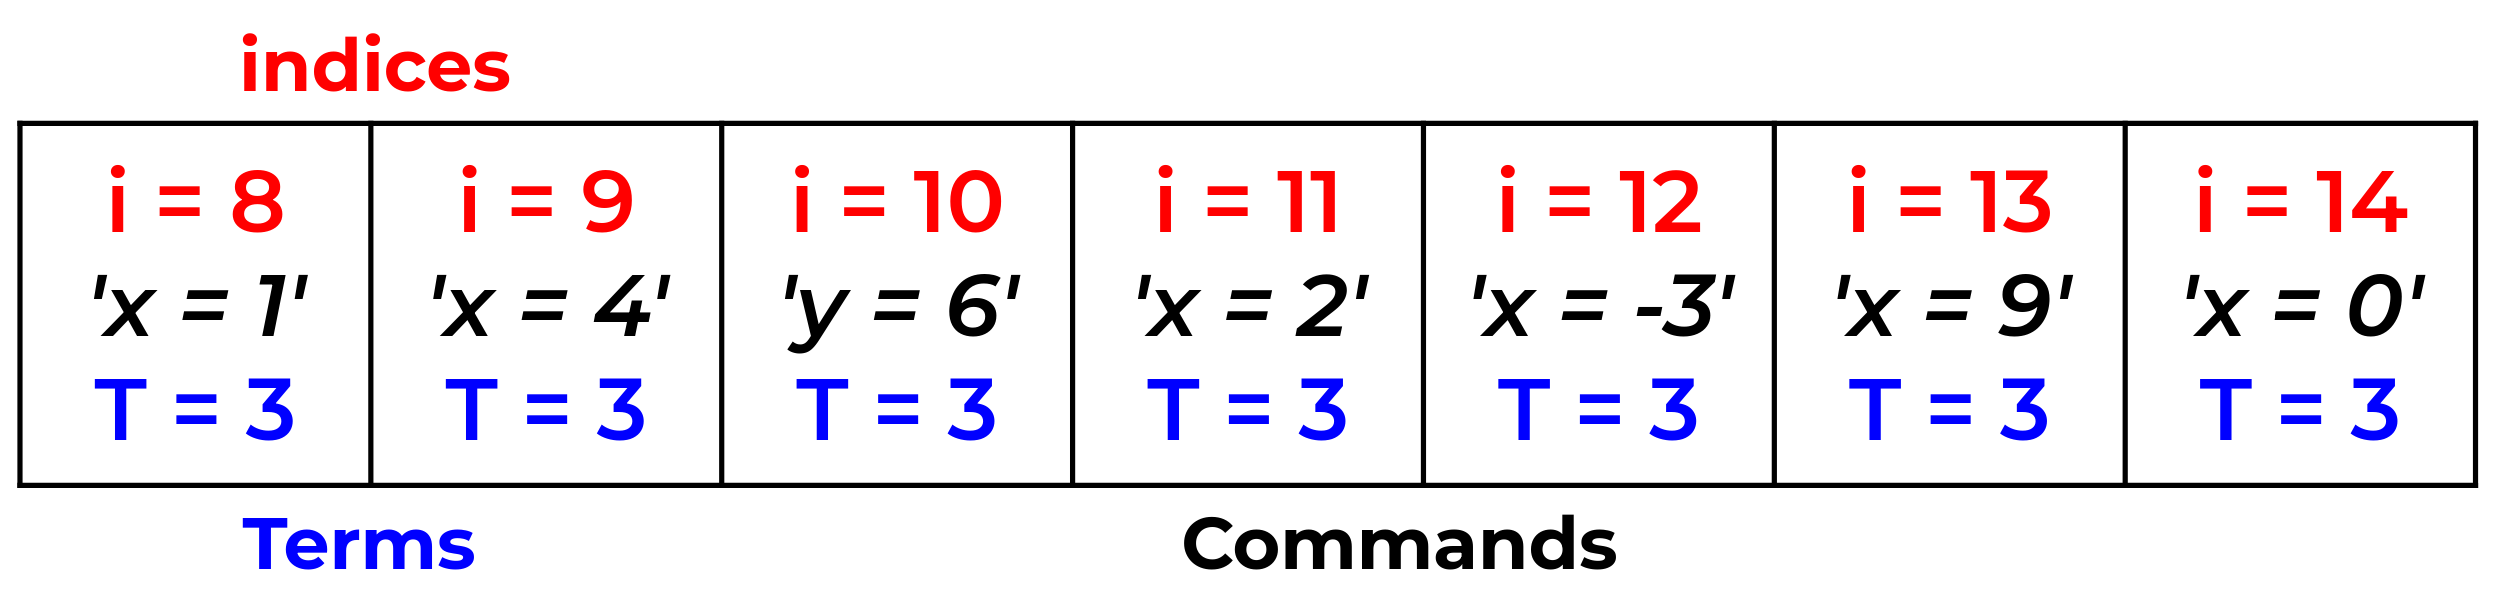
\includegraphics[width=.8\linewidth]{images/logStructure.png}
  
  \caption{Raft's log is fundamentally an array made of entries.}
  \Description{An array, thus a list of consecutive elements, each of which is an entry with its own index, term and data.}
  \label{fig:logStructure}
\end{figure}

\subsection{Log Replication and Overwriting}

All log propagation revolves around one core remote procedure call named \textit{append\_entries\_rpc}, which the leader calls on a list of server proxies that connects it to the followers, which in turn call on a proxy of the leader. It must be registered in the server to be callable, as can be seen in listing \ref{code:registerFunction}.

\begin{python}[label={code:registerFunction}, caption={Register, thus making it callable, the remote procedure call \textit{append\_entries\_rpc}}]
def handle_server():                                    # enclose server in a callable function
    with Raft(...) as server:                           # creates SimpleXMLRPCSever
        def append_entries_rpc(entries, term, commit_index, all_log):
            # ...
        server.register_function(append_entries_rpc)    # makes function callable on the other side
        server.serve_forever()                          # keeps server alive 
\end{python}

\subsubsection{Leader Propagates Entries} \label{sec:leaderSends}

The leader (each server as a matter of fact) periodically checks whether there are new commands to propagate (always stored in queue \textit{pygame\_commands}), by overriding \textit{SimpleXMLRPCServer}'s method \textit{service\_actions} (listing \ref{code:addCommands}, more details in section \ref{sec:raftian}).

Then, translates them into entries by giving each of them the current term and a log index that starts from $lastLogEntry(index) + 1$ and increases by one for each entry. To give an example: if $lastLogEntry(index) = 7$ and we have three new commands, their indexes will respectively be eight (8), nine (9) and ten (10). The translation can be seen at listing \ref{code:translateCommands}

At this point it propagates \textit{new\_entries} to the whole cluster, updating the commit index (necessary for applying log to state) as soon as propagations are successful on at least half of the cluster, like so: $commitIndex = lastNewEntry(index)$. 

What happens if the \textit{append entries} gets rejected? The leader adds to \textit{new\_entries} its own last log entry: $new\_entries = lastLogEntry + new\_entries$ (figure \ref{fig:newEntries}). Then repeats the propagation procedure, for each reject a new \textit{last log entry} gets added, progressively traversing the log backwards. If, at a certain point, $new\_entries == allLog + new\_entries$ (i.e., all leader's log gets propagated) the flag \textit{all\_log} is set to \textit{True}. 

Since every server may reject or accept different sets of entries, depending on their own local log, every propagation must be "local" for each follower. 

The flow of execution for the log propagation is: \textit{Raft: service\_actions} \faArrowRight\ \textit{Raft: propagate\_entries} \faArrowRight\ \textit{propagate\_entries} \textit{:encapsulates\_proxy:} \textit{append\_entries\_rpc}. The last one gets called as many times as needed on every single follower.

Of course, all propagation happens concurrently using a \textit{ThreadPoolExecutor}, and the code for entries propagation (leader's side) can be seen at listing \ref{code:leaderPropagateEntries}.

\begin{figure}[h]
  \centering
  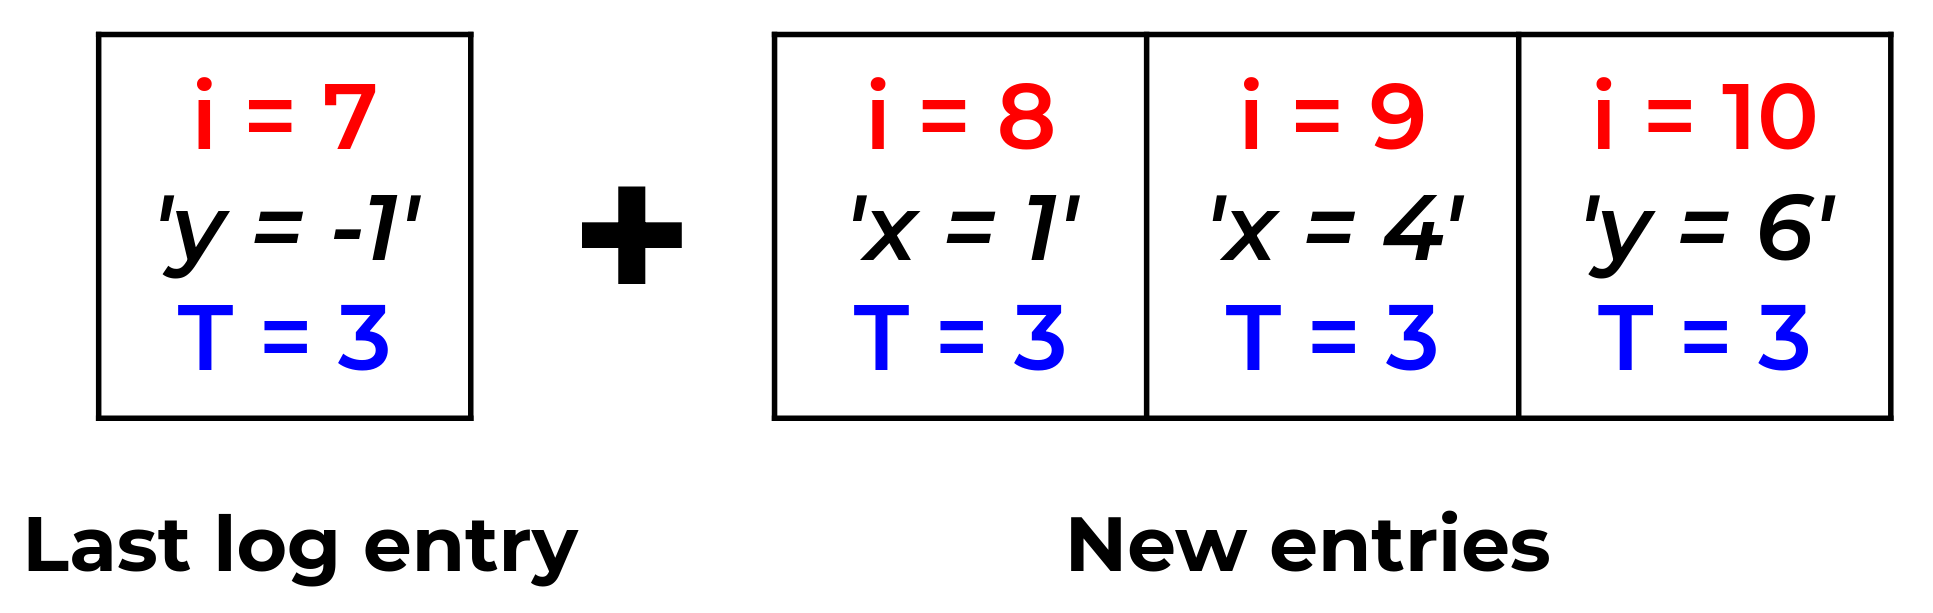
\includegraphics[width=.8\linewidth]{images/newEntries.png}
  
  \caption{New entries with the last log's entry added to the beginning of the list.}
  \Description{Two arrays, where the first is only one element (the last log's entry) which gets added at the beginning of the second array, i.e., the new entries.}
  \label{fig:newEntries}
\end{figure}

\begin{python}[label={code:addCommands}, caption={Periodically checks whether there are new commands}]
def service_actions(self):                      # RUN method of the server, override
    if time.time() - self.countdown >= .005:    # do actions every .005 seconds
        global pygame_commands

        if not pygame_commands.empty():         # propagate entries to cluster
            self.propagate_entries()
\end{python}

\begin{python}[label={code:translateCommands}, caption={Translates commands into new entries}]
def propagate_entries():
# ...
    while not pygame_commands.empty():
        command = pygame_commands.get()
        log_index += 1                          # lastLogEntry(index) + 1
        self.new_entries.append(Raft.Entry(     # append to support list 'new_entries'
            term=self.term,
            index=log_index,
            command=command
        ))
\end{python}

\begin{python}[label={code:leaderPropagateEntries}, caption={Leader propagation procedure, for complete code refer to project's repository}]
def propagate_entries(self):        
    # ...          
    if self.log:                            # travel backwards through self.log for each reject
        entries: list[Raft.Entry] = []
        entries.append(self.log[-1])    
        entries.extend(self.new_entries)    
        log_iterator: int = -2              # log_iterator soft resets for each follower
    else:
        entries: list[Raft.Entry] = self.new_entries
        log_iterator: int = -1
        
    # ...
    # inner function necessary for concurrent execution
    def encapsulate_proxy(self, follower, entries, log_iterator):
        # ...
        with xmlrpc.client.ServerProxy(complete_url, allow_none=True) as proxy: 
            while not propagation_successful:
                # send new entries (local for each follower) 
                # ...
                result = proxy.append_entries_rpc(entries, self.term, self.commit_index, all_log)
                if result[0] == False:
                    # add another entry from self.log to new entries
                    entries = [self.log[log_iterator]] + entries 
                    log_iterator -= 1   
                elif result[0] == True:
                    propagation_successful = True

        return propagation_successful # to propagate_entries, make propagation counter increase 
        # encapsulate_proxy ends

    results = []

    # fires RPCs concurrently using ThreadPoolExecutor 
    future_result = {           # clever python syntax trick 
        self.executor.submit(
            encapsulate_proxy,  # function
            self,               # function's parameter
            follower,           # function's parameter
            entries,            # function's parameter
            log_iterator        # function's parameter
            ): follower for follower in self.cluster}
    for future in concurrent.futures.as_completed(future_result):
        # results of RPCs
        data = future.result()
        results.append(data)

    # finally counts if propagation was successful enough
    if results.count(True) >= len(self.cluster) / 2:
        self.log.extend(self.new_entries)               # add new entries to log
        self.new_entries.clear()                        # clear new entries list
        self.commit_index = self.log[-1].index          # ensure log gets eventually applied
    else:
    #   new entries are not cleared, so they will be propagated again
\end{python}

\subsubsection{Follower Recieves Entries}

When a follower receives an \textit{append entries} request from the leader, first checks whether leader's term is up to date. If it's not, i.e., $leaderTerm < followerTerm$, rejects by answering with the tuple $(False, followerTerm)$. In this context, \textit{answering} is done via the remote procedure call's return value.

If, on the other hand, the leader's term is equal or greater than its own (i.e., $leaderTerm \geq followerTerm$), the follower updates its commit index and, if $leaderEntries \neq \emptyset$, checks the \textit{all\_log} flag. If it's \textit{True}, clears all its own log to overwrite it with the leader's (fundamental to log forcing, listing \ref{code:clearLog}). Otherwise ($all\_log \neq True$), the leader did not send all its log, so the follower searches through its own log for an entry equal to the leader's previous one (i.e., the entry preceding the new ones). Let's make an example: 

\begin{itemize}
    \item Leader's log = $[1, 2, 3, 4, 5]$;
    \item Leader's new entries = $[6, 7]$;
    \item Thus leader's prev = $[5]$.
\end{itemize}

If it finds an entry equal to leader's previous (i.e., $followerLog(someEntry) == leaderPrev$), deletes all log entries that follow it and appends new ones, otherwise ($\nexists(followerLog(someEntry) == leaderPrev)$) rejects the request. Since the leader, when faced with a reject, adds a new \textit{prev} and keeps repeating the send until it comprises all its log, at a certain point the follower will be forced to overwrite all its log, thus making it equal to the leader's. This overwriting is called \textit{log forcing} and ensures that all logs are equal to the leader's.

The code can be seen at listing \ref{code:searchFollowerLog} (for the complete one refer to the repository).

\begin{python}[label={code:clearLog}, caption={Follower clears its own log to overwrite it with the leader's}]
if all_log == True:
    server.log.clear() # if leader sent all its log, clear and rewrite log (leader's log forcing)
\end{python}

\begin{python}[label={code:searchFollowerLog}, caption={Follower search in its own log for an entry equal to leader's prev}]
if commit_index is not None:                    
        server.commit_index = commit_index  # update commit index 

if entries is not None:     # not an heartbeat
    if all_log == True:     # complete overwrite
        server.log.clear()

    if server.log:  # if follower's log not empty search for an entry equal to leader's prev
        entry_log_index: int | None = None              # save its log index (!= entry index)
        for i, my_entry in enumerate(server.log):
            if (my_entry.index == entries[0].index 
                and my_entry.term == entries[0].term):
                entry_log_index = i
                break # no need to search further
        # here entry_log_index == (position of entry equal to leader.prev) | None

        if entry_log_index is None:         # entry equal to leader's prev not found
            return(False, server.term)      # rejects

        del server.log[(entry_log_index ):] # delete all log following leader prev 

    server.log.extend(entries) # append new entries
\end{python}

\subsubsection{Follower Sends Entries}

Since every server is a Raftian node with a game instance and thus player inputs, followers have their own Pygame commands to propagate. Just like the leader, in their \textit{service\_actions} function they periodically check whether there are new commands to propagate and call \textit{propagate\_entries} accordingly. Then, they translate all Pygame commands into entries (same code as listing \ref{code:translateCommands}) and propagate them to the leader via \textit{append\_entries\_rpc}. Nothing else. 

As previously stated, followers are \textit{passive}, meaning they do not apply their own player inputs when they register them, but only after the leader propagates them back to the whole cluster.

\subsubsection{Leader Receives Entries}

The leader does very little when receives entries from the followers: it just puts them into its own \textit{pygame\_commands} queue. They will get processed and propagated eventually, as stated in section \ref{sec:leaderSends}.

\subsection{Apply Log to State}

Let's first explain two key attributes: \textit{commit index} and \textit{last applied}. Both of these represent an index, but the former is the highest-index entry successfully propagated in the cluster, while the latter is the highest-index entry already applied to state. 

Every node, whether leader or follower, applies entries to state in the same way: inside their function \textit{service\_actions} they periodically check if there is a discrepancy between \textit{commit index} and \textit{last applied} attributes (i.e., $commit\_index > last\_applied$). Then, starting from the last applied entry, they apply to state all successive entries up to and including the one with the same index as \textit{commit\_index}, updating \textit{last\_applied} as they go. To clarify: servers apply all entries between $log(entry.index == last\_applied)$ and $log(entry.index == commit\_index)$ as shown in figure \ref{fig:applyToState}. 

To apply entries in our context means that they get appended to the queue \textit{raft\_orders}. The code can be seen at listing \ref{code:applyToState} (for the complete source refer to the repository)

\begin{figure}[h]
  \centering
  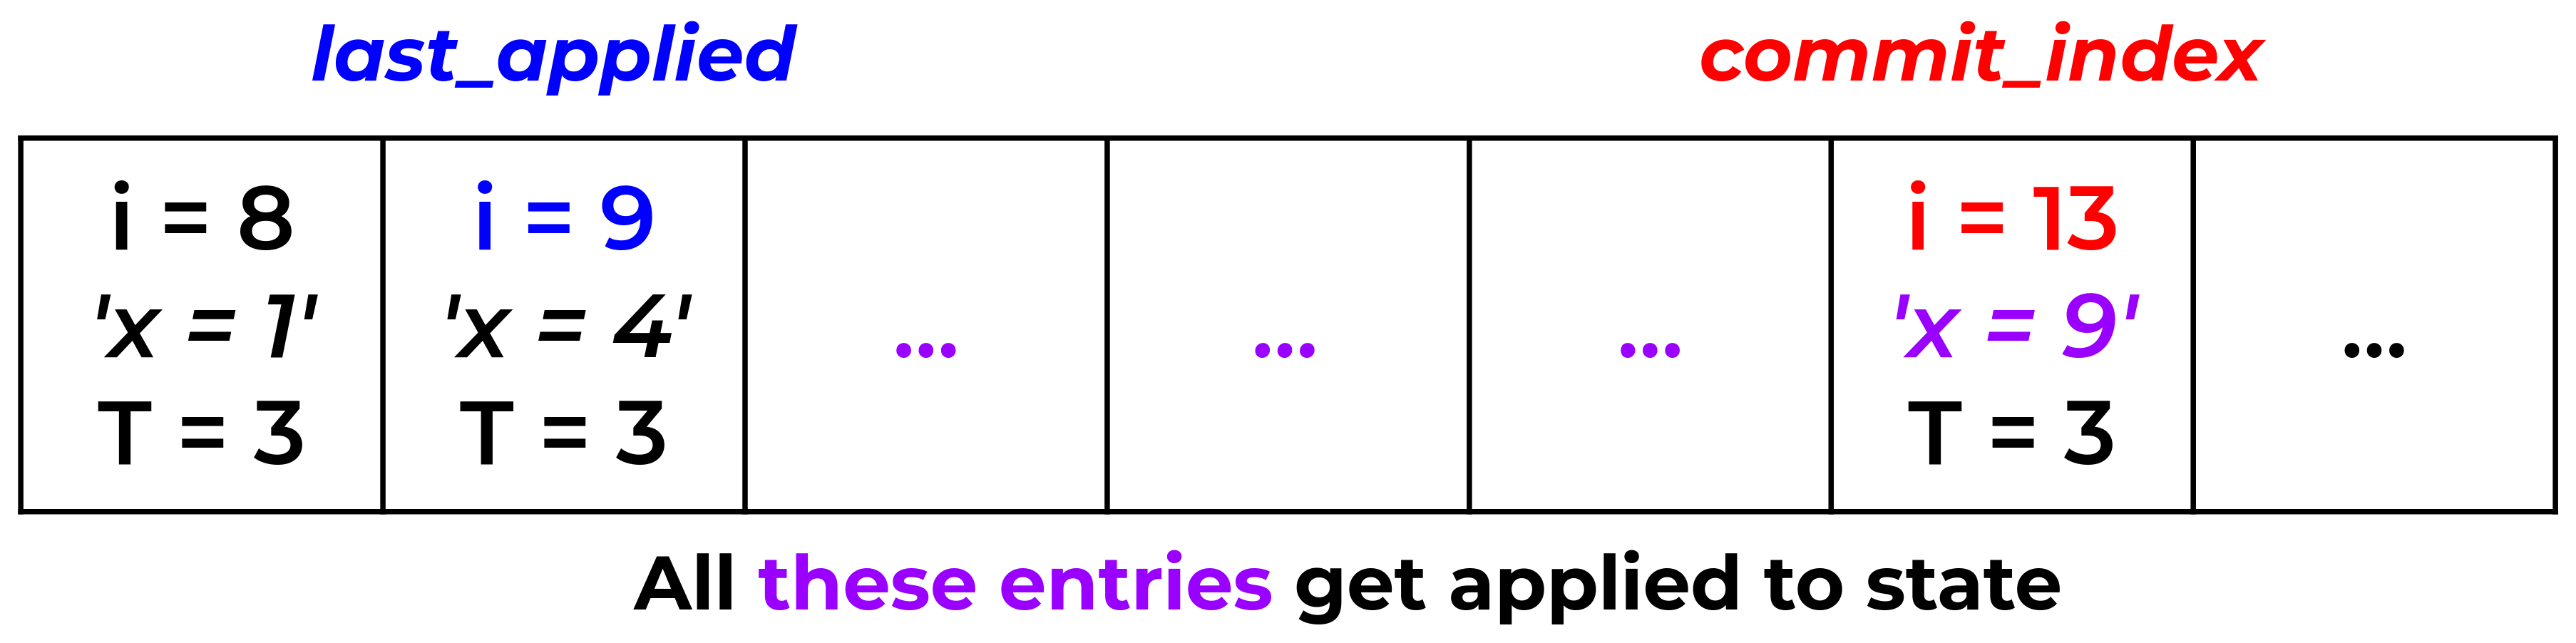
\includegraphics[width=.8\linewidth]{images/applyToState.png}
  
  \caption{All entries between \textit{last\_applied} and \textit{commit\_index} (included) get applied to state.}
  \Description{An array showing that all entries between the last applied and the last committed get applied to state.}
  \label{fig:applyToState}
\end{figure}

\begin{python}[label={code:applyToState}, caption={All nodes apply entries to state based on \textit{commit\_index}}]
def service_actions(self):
        # ...
        if self.commit_index is not None and self.commit_index > self.last_applied:   
            global raft_orders  # applying means appending entries to this queue

            #...

            last_applied_log_position: int = -1 
            for i, my_entry in enumerate(self.log):
                if (my_entry.index == self.last_applied):
                    last_applied_log_position = i
                    break # found log position of last applied entry 
            
            log_iterator = last_applied_log_position + 1    # improves code clarity 

            while self.last_applied != self.commit_index:
                raft_orders.put(self.log[log_iterator])
                self.last_applied = self.log[log_iterator].index
                log_iterator = log_iterator + 1
            # here self.last_applied == self.commit_index
\end{python}

\subsection{Log Compaction}

\subsection{Leader Election}

\subsection{Cluster Membership Change}

\subsection{Byzantine Raft}

%%
%% The acknowledgments section is defined using the "acks" environment
%% (and NOT an unnumbered section). This ensures the proper
%% identification of the section in the article metadata, and the
%% consistent spelling of the heading.
\begin{acks}
To Robert, for the bagels and explaining CMYK and color spaces.
\end{acks}

%%
%% The next two lines define the bibliography style to be used, and
%% the bibliography file.
\bibliographystyle{ACM-Reference-Format}
\bibliography{report}


%%
%% If your work has an appendix, this is the place to put it.
\appendix

\section{Appendix Section}

Etiam commodo feugiat nisl pulvinar pellentesque. Etiam auctor sodales
ligula, non varius nibh pulvinar semper. Suspendisse nec lectus non
ipsum convallis congue hendrerit vitae sapien. Donec at laoreet
eros. Vivamus non purus placerat, scelerisque diam eu, cursus
ante. Etiam aliquam tortor auctor efficitur mattis.

\subsection{Appendix Subsection}

Etiam commodo feugiat nisl pulvinar pellentesque. Etiam auctor sodales
ligula, non varius nibh pulvinar semper. Suspendisse nec lectus non
ipsum convallis congue hendrerit vitae sapien. Donec at laoreet
eros. Vivamus non purus placerat, scelerisque diam eu, cursus
ante. Etiam aliquam tortor auctor efficitur mattis.

\end{document}
\endinput
%%
%% End of file `sample-manuscript.tex'.
